\section{Likelihood details and calibration contract}
\label{app:likelihood}

The joint likelihood sums DESI DR2 BAO terms with published
covariances, the compressed CMB prior used during endpoint discovery,
and the Pantheon+SH0ES joint term. No external $H_{0}$ prior enters
the likelihood.

Pantheon+SH0ES is one 1657-row covariance likelihood with one common
profiled $M$. With $r_{0}=m_{B}^{\mathrm{corr}}-\mu_{\mathrm{no}\,M}$,
\begin{equation}
  \hat{M} = \frac{\mathbf{1}^{T}C^{-1}r_{0}}
                 {\mathbf{1}^{T}C^{-1}\mathbf{1}},
  \qquad
  \chi^{2}_{\mathrm{joint}}
    = (r_{0}-\hat{M}\mathbf{1})^{T}C^{-1}(r_{0}-\hat{M}\mathbf{1}),
\end{equation}
where $C$ is the full $1657\times1657$ covariance. Ladder and
non-ladder blocks are diagnostics: each uses its marginal covariance
with an independent $M$, so
$\chi^{2}_{\mathrm{ladder}}+\chi^{2}_{\mathrm{non\text{-}ladder}}
\neq \chi^{2}_{\mathrm{joint}}$.

Calibrator rows use $\mu_{\mathrm{cal}}=\mathrm{CEPH\_DIST}$.
Under the adopted calibration contract, no additional theory-side
correction is applied to local calibrator distance moduli:
$\Delta\mu_{\mathrm{cal}}=0$; this covers the declared contract only
and is a qualitative assumption, not quantitatively established.
Hubble-flow rows use $z_{\mathrm{HD}}$
for $D_{M}$ and the $z_{\mathrm{HD}}$/$z_{\mathrm{HEL}}$ prefactor
$D_{L}=(1+z_{\mathrm{HEL}})D_{M}(z_{\mathrm{HD}})$, which assumes massless
photons, null geodesics, and photon-number conservation
\citep{Etherington1933}.

The endpoint-discovery CMB block is the compressed set
$(R,\ell_{A},\omega_{b}h^{2})$ with numerical values from
\citep{Chen2019}, validated there against conventional late-time
models only:
\begin{equation}
  D_{M}(z_{*})=c\,I(z_{*})\,r_{d}/(100\,h_{\mathrm{rd}}),
  \qquad
  \ell_{A}=\pi D_{M}(z_{*})/r_{s}.
  \label{eq:app-cmb-prior}
\end{equation}
This is a compressed
$R,\ell_{A},\omega_{b}h^{2}$ prior, not a TT/TE/EE likelihood, and it
cannot by itself validate nonstandard pre-recombination physics for
R. The C1/C2 reference constructions are calibrated directly to the
full Planck spectra (Section~\ref{sec:data}).

\subsection{Calibration contract}
No telescope or catalog data were rescaled. All changes are in the
forward model, not the data: observed redshifts, magnitudes,
covariances, masks, and Cepheid distances are untouched.

DESI path: $z_{\mathrm{obs}}\to z_{\mathrm{bg}}\to
D_{M},D_{H},D_{V}\to D/r_{d}$ with each endpoint's own ruler from
Table~\ref{tab:calibration}; observed
$D/r_{d}$ rows and published covariances are unchanged.
Pantheon+SH0ES path: 1657 selected rows including 77 calibrators;
$z_{\mathrm{HD}}$ for cosmological distance, $z_{\mathrm{HEL}}$ in
the luminosity prefactor, CEPH\_DIST for calibrator $\mu$; one
common profiled $M$ with full $1657\times1657$ covariance in the fit;
source-defined ladder split is diagnostic-only with independent $M$
terms and is non-additive under the joint cross-covariance.

\begin{figure}[!htbp]
\centering
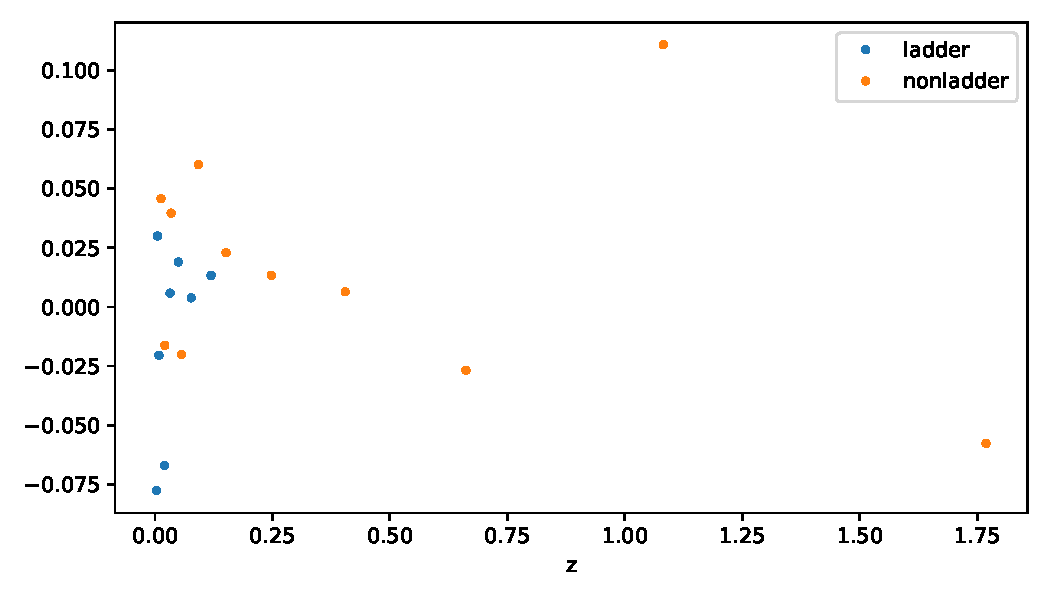
\includegraphics[width=0.9\linewidth]{figures/generated/figure_A_sn_subset_diagnostics.pdf}
\caption{Appendix-only subset-profiled supernova diagnostics:
source-defined ladder diagnostic, independently profiled $M$ (left) and
complementary non-ladder diagnostic, independently profiled $M$ (right).
Non-additive; never used in the joint fit.}
\label{fig:sn-subset}
\end{figure}
